\def\assignmenttitle{Assignment 1}
\def\assignmentdate{16-10-2011}
\def\assignmentnumber{1}

\documentclass[11pt]{article}
\linespread{1}

\renewcommand{\thefootnote}{\fnsymbol{footnote}}

\usepackage{geometry} % see geometry.pdf on how to lay out the page. There's lots.
\usepackage[utf8]{inputenc}
\usepackage{array}
\usepackage{amsmath,amssymb,latexsym,epic,eepic,epsfig,graphics,psfrag}
\usepackage{amsfonts}
\usepackage{graphicx,float}

\usepackage[danish]{babel}

\usepackage[bottom]{footmisc}

\usepackage{fancyhdr}
\pagestyle{fancy}
\lhead{\small\textit{01246 Partial Differential Equations - Fall 2011 - Anders Hørsted (s082382)}}
\rhead{\thepage}
\chead{}
\lfoot{}\cfoot{}\rfoot{}

\usepackage{pstricks}
\usepackage{pst-node}
\usepackage{wrapfig}
\usepackage{caption}
\usepackage{multirow}
%\usepackage{fouriernc}
%\usepackage[charter]{mathdesign}
\usepackage{lmodern}
\usepackage[normalem]{ulem}
\geometry{a4paper} % or letter or a5paper or ... etc
% \geometry{landscape} % rotated page geometry

\usepackage{subfigure}
\usepackage{placeins}
\usepackage{url}
\usepackage{natbib}
\renewcommand\bibsection*{}
\bibliographystyle{plain}

\makeatletter
\renewcommand*\env@matrix[1][*\c@MaxMatrixCols c]{%
  \hskip -\arraycolsep
  \let\@ifnextchar\new@ifnextchar
  \array{#1}}
\makeatother

\newcommand\myimp{\quad\Leftrightarrow\quad}
\newcommand\half{\frac{1}{2}}
%\newcommand\myvec[1]{\mathbf{#1}}
\newcommand\myvec[1]{\boldsymbol{#1}}
\newcommand\vecx{\myvec{x}}
\newcommand\mymod[1]{\ (\text{mod }#1)}
\newcommand\myreal{\mathbb{R}}
\newcommand\mynatural{\mathbb{N}}
\newcommand\myinteger{\mathbb{Z}}
\newcommand\mycomplex{\mathbb{C}}
\newcommand\myint{\text{int}}
\newcommand\norm[1]{||\,#1\,||}
\newcommand\bignorm[1]{\big|\big|\,#1\,\big|\big|}
\newcommand\seq[1]{\big\{#1\big\}}
\newcommand\smallseq[1]{\{#1\}}
\newcommand\smallseqtoinf[1]{\smallseq{#1}_{k=1}^\infty}
\newcommand\lonew{\ell^1_w}
\newcommand\lone{\ell^1}
\newcommand\ltwo{\ell^2(\mynatural)}
\newcommand\ip[2]{\langle#1,#2\rangle}
\newcommand\hilbert[1]{\mathcal{#1}}
\newcommand\uinf{u_{\infty}}
\newcommand\erf{\text{erf\,}}
\newcommand\infint{\int_{\infty}^{\infty}}
\newcommand\celsius{$^\circ$C}
\newcommand\comsol{Comsol}
\newcommand\fourier{\mathcal{F}}

\usepackage{tabulary}
\newcolumntype{y}{>{\centering\arraybackslash}R}

\setlength{\unitlength}{2mm}
\usepackage{tikz}

\title{Homework \homeworknumber}
\author{01246 Partial differential equations -- \homeworkdate -- Anders Hørsted (s082382)}
%\author{}
\date{} % delete this line to display the current date


\begin{document}

\maketitle

\section*{Question 1 - Branin's function}
Branin's function $\myvec{r}\,:\,\myreal^2\to\myreal^2$ is defined as
\begin{align}
    r_1(\myvec{x}) &= 1 - 2x_2 + \frac{1}{20}\sin(4\pi x_2) - x_1 \nonumber\\
    r_2(\myvec{x}) &= x_2 - \frac{1}{2}\sin(2\pi x_1)\label{eq:branin}
\end{align}
and the function $f$ is then defined as
\begin{equation}\label{eq:braninsq}
    f(\myvec{x}) = \half(r_1(\myvec{x})^2 + r_2(\myvec{x})^2)
\end{equation}
\subsection*{Question 1.1}
Since the function $f$ is defined as the sum of two squared values we have that $f(\myvec{x})\geq 0$ for all $\myvec{x}\in\myreal^2$ and only for $r_1(\myvec{x})=r_2(\myvec{x})=0$ is $f(\myvec{x})=0$. From this it is seen that any solution of $\myvec{r}(\myvec{x})=\myvec{0}$ is also a minimizer of $f$.

\subsection*{Question 1.2}
A contour plot of $\log_{10}(f(\myvec{x}))$ for $\myvec{x}\in[-10;10]\times[-10;10]$ is plotted and shown in figure~\ref{fig:q12}
\begin{figure}
    \centering
    \includegraphics[width=90mm]{q12-crop.pdf}
    \caption{Contour plot of $\log_{10}f(\myvec{x})$ as defined in question 1.}
    \label{fig:q12}
\end{figure}

\pagebreak

\section*{Question 2 - Newton's Method}
\subsection*{Question 2.1}
First an \textsc{Matlab} implementation of Newton's method is created.
\lstinputlisting[caption={Implementation of Newton's method},label=lst:newton,language=Matlab]{Newton.m}

\subsection*{Question 2.2}
The implementation is tested on the quadratic function $f(\myvec{x}) = \half\myvec{x}^T\myvec{Ax} + \myvec{b}^T\myvec{x}$ where
\begin{equation*}
    \myvec{A} = \begin{pmatrix}
        2 & 1 \\
        1 & 2
    \end{pmatrix}, \quad \myvec{b} = \begin{pmatrix}
        -1.5 \\
        0
    \end{pmatrix}
\end{equation*}
The extremum $\myvec{x}^*$ can be found analytically by using $\nabla f(\myvec{x}) = \myvec{Ax} + \myvec{b}$, which gives
\begin{align*}
    \myvec{Ax}^* + \myvec{b} = 0 \myimp
    \myvec{x}^* = -\myvec{A}^{-1}\myvec{b} = \begin{pmatrix}
        1 \\
        -0.5
    \end{pmatrix}
\end{align*}
Using the implementation of Newton's method we find the same minimizer as the analytical solution, and Newton's method uses only one iteration. This is as expected since the first iteration $\vecx^{(1)}$ is given by (using that $\nabla^2 f(\vecx) = \vecA$)
\begin{align*}
    \vecx^{(1)} &= \vecx^{(0)} - \vecA^{-1}(\vecA\vecx^{(0)}+\myvec{b}) \myimp\\
    \vecA\vecx^{(1)} + \vecA\vecx^{(0)} + \myvec{b} &= \vecA\vecx^{(0)} \myimp\\
    \vecx^{(1)} &= -\vecA^{-1}\myvec{b}
\end{align*}
so $\vecx^*=\vecx^{(1)}$ for the quadratic function $f$.

\subsection*{Question 2.3}
Now the implementation of Newton's method is tested\footnote{Using a tolerance of $10^{-12}$ and a maximum of 1000 iterations.} on $f$ -- as defined in (\ref{eq:braninsq}) -- for four different starting guesses: $\vecx^{(0)}_{1}=(0,0)^T, \vecx^{(0)}_{2}=(1,0)^T, \vecx^{(0)}_{3}=(3.9, -1)^T, \vecx^{(0)}_{4}=(4.1, -1)^T$. The results are shown in figure~\ref{fig:newton-test}. For the first three starting guesses the algorithm converges within the first 10 iterations giving the minimizers
\begin{equation*}
    \vecx_1^{(8)} = \begin{pmatrix}
        0.1487 \\ 0.4021
    \end{pmatrix}, \quad
    \vecx_2^{(0)} = \begin{pmatrix}
        1 \\ 0
    \end{pmatrix}, \quad
    \vecx_3^{(6)} = \begin{pmatrix}
        3.7305 \\ -1.2306
    \end{pmatrix}
\end{equation*}
but for the starting guess $\vecx_4^{(0)}$ the algorithm do not converge within the allowed 1000 iterations. The reason for the lack of convergence can be found by inspecting the last few iterations. For the last 4 iterations the $\vecx$ values are
\begin{equation*}
    \vecx_4^{(997)} = \begin{pmatrix}
        13.5082 \\ -2.3639
    \end{pmatrix}, \quad 
    \vecx_4^{(998)} = \begin{pmatrix}
        13.5629 \\ -2.5779
    \end{pmatrix}, \quad 
    \vecx_4^{(999)} = \begin{pmatrix}
        13.5082 \\ -2.3639
    \end{pmatrix}, \quad 
    \vecx_4^{(1000)} = \begin{pmatrix}
        13.5629 \\ -2.5779
    \end{pmatrix}
\end{equation*}
and it do look like the algorithm is cycling between two different $\vecx$ values. Closer inspection of the $\vecx$ values shows that this is indeed the case. \par
It is now tested whether the found minimas are solutions for $\myvec{r}(\vecx)=0$ or only local minimizers for $f(\vecx)$. For $\vecx_2^{(0)}=(1,0)^T$ it is seen from the expression (\ref{eq:branin}) that it is a solution. For the other three candidates the norms of $\myvec{r}$ are calculated as
\begin{gather*}
    \norm{\myvec{r}(\vecx_1^{(8)})}_2 = 2.78\cdot 10^{-17}, \quad 
    \norm{\myvec{r}(\vecx_3^{(6)})}_2 = 7.86\cdot 10^{-1}, \quad\norm{\myvec{r}(\vecx_4^{(1000)})}_2 = 7.82
\end{gather*}
Which shows that $\vecx_1^{(8)}$ is a solution, but $\vecx_3^{(6)}$ and $\vecx_4^{(1000)}$ are ony local minimizers of $f$.
\begin{figure}
    \centering
    \mbox{\subfigure{\includegraphics[width=70mm]{newton-on-branin-1-crop.pdf}} \quad \subfigure{\includegraphics[width=70mm]{newton-on-branin-2-crop.pdf}}}
    \mbox{\subfigure{\includegraphics[width=70mm]{newton-on-branin-3-crop.pdf}} \quad \subfigure{\includegraphics[width=70mm]{newton-on-branin-4-crop.pdf}}}
    \caption{Testing implementation of Newton's method shown in code~listing~\ref{lst:newton}}
    \label{fig:newton-test}
\end{figure}

\section*{Question 3 - Least Squares Methods}
In this question different function will be fitted to a dataset containing measurements of light intensity in a optical fibre as a function of time after source cut off.

\subsection*{Question 3.1}
First polynomials of degrees from 1 to 6 are fitted to the data using the \matlab\ function \myverb{polyfit}. The results are shown in figure~\ref{fig:gitted-polynomials} and from the figure it is seen that the fit can be improved for values inside the data interval, by raising the degree of the polynomial. This is as expected since we could make the polynomial fit the data exactly by choosing the degree equal to the number of datapoints minus one (as long as there aren't two measurements for the same $t$). Outside the data interval though the behaviour of the fitted polynomials do not behave as well since all polynomials makes a sharp upward or downward turn when $t>32$. This behaviour do not match the physical reality well, so instead of using polynomials, exponential functions are fitted instead.
\begin{figure}
    \centering
    \mbox{\subfigure{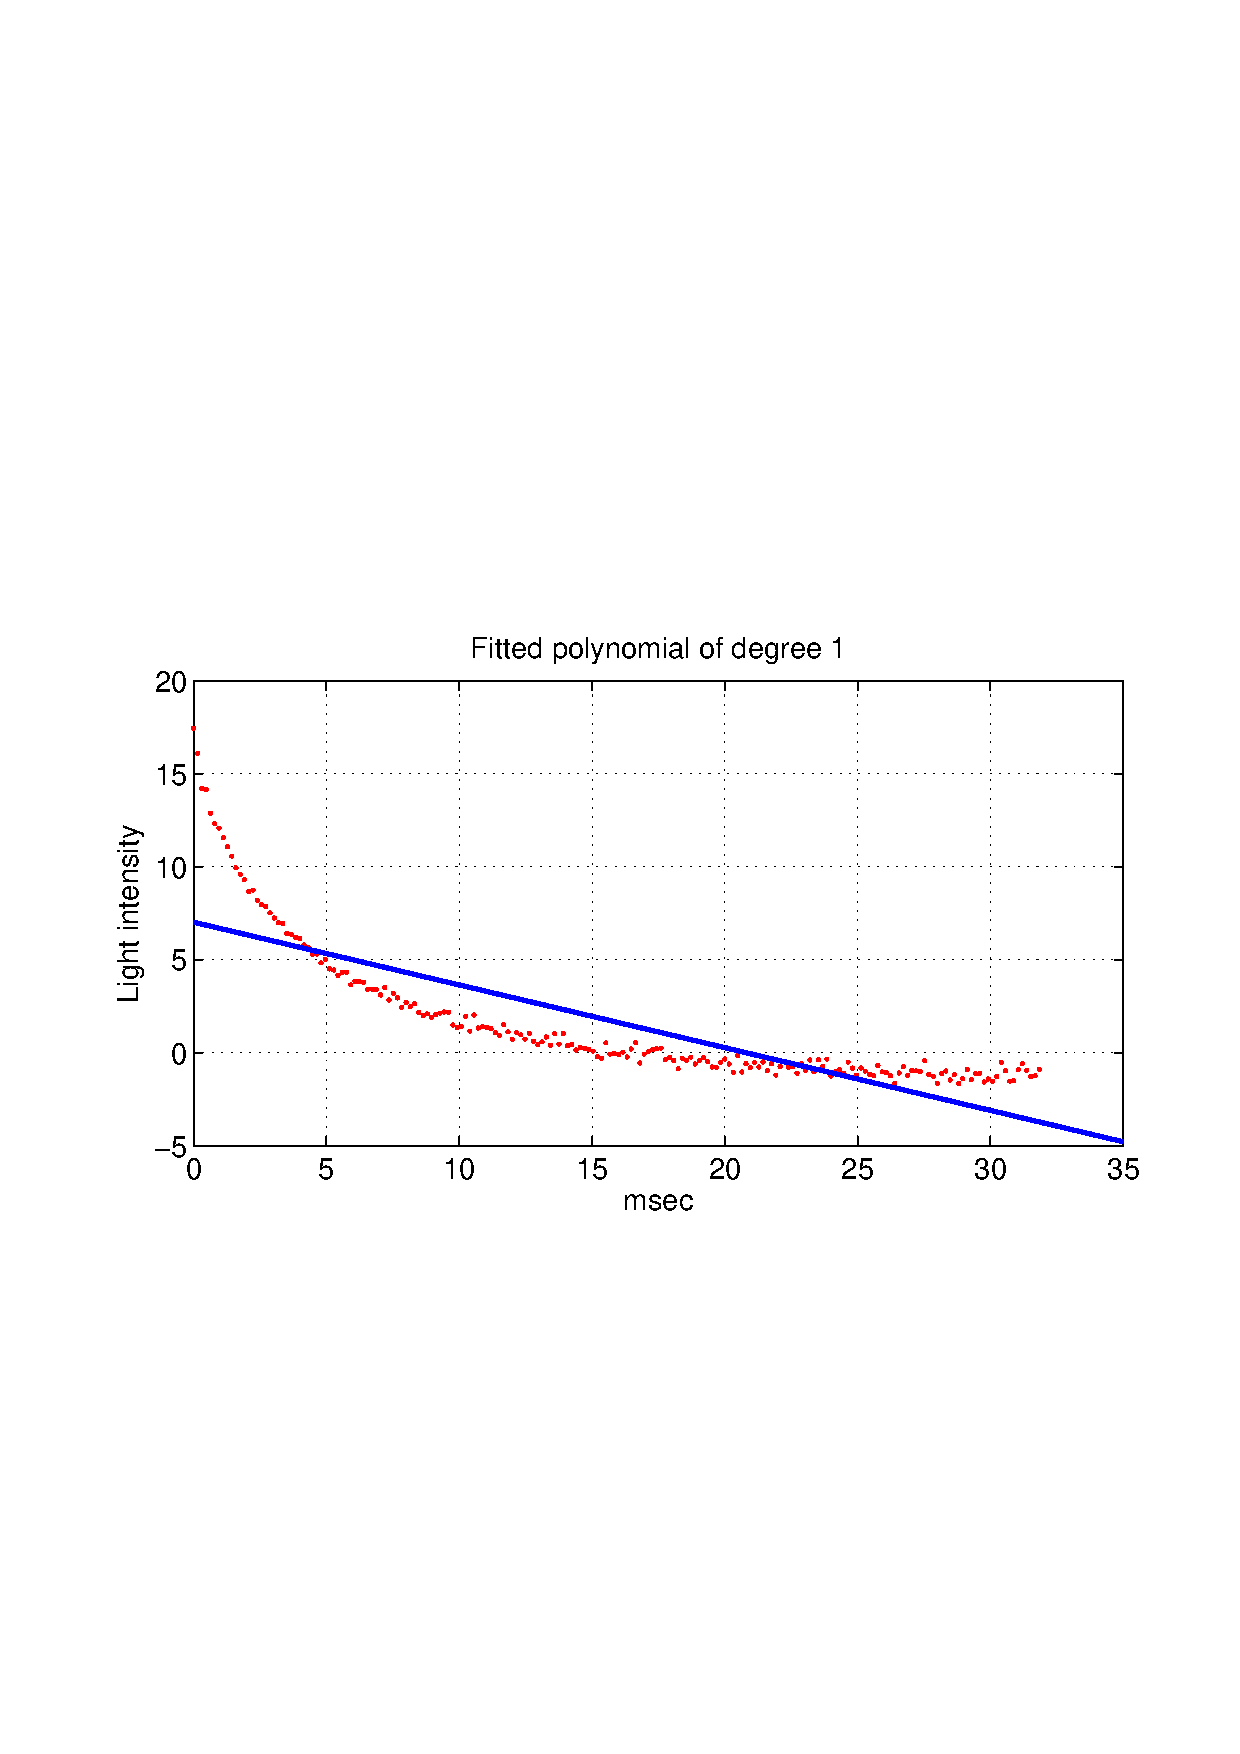
\includegraphics[width=70mm]{fitted-polynomial-1.pdf}} \quad \subfigure{\includegraphics[width=70mm]{fitted-polynomial-2.pdf}}}
    \mbox{\subfigure{\includegraphics[width=70mm]{fitted-polynomial-3.pdf}} \quad \subfigure{\includegraphics[width=70mm]{fitted-polynomial-4.pdf}}}
    \mbox{\subfigure{\includegraphics[width=70mm]{fitted-polynomial-5.pdf}} \quad \subfigure{\includegraphics[width=70mm]{fitted-polynomial-6.pdf}}}
    \caption{Fitted polynomials of degrees 1 to 6.}
    \label{fig:fitted-polynomials}
\end{figure}

\subsection*{Question 3.2}
Now the data $\{(t_i, y_i)\}_{i=1}^m$ is fitted by the model
\begin{equation}\label{eq:model1}
    M(x, t) = x_2 e^{-x_1t} + x_3
\end{equation}
First a function returning the residual vector and the jacobian matrix for the data given the parameters $\vecx$ as input is implemented. To make the function more generic we let it receive the data \myverb{t} and \myverb{y} as second and third argument. The actual data can then be passed in to the \myverb{marquardt} function.
\lstinputlisting[caption={Function returning value of model 1}]{M1.m}
\lstinputlisting[caption={Function returning residual vector and jacobian for a given data set}]{residual_jacobian_M1.m}
The actual model is defined in a separate function \myverb{M1} since it is going to be reused when plotting the model. To ensure that the function is correctly implemented it is checked by running the \myverb{checkgrad} function.
\begin{lstlisting}
[maxJ, err, ind] = checkgrad(@residual_jacobian_M1, x0, 1e-5, t, y);
\end{lstlisting}
The function returns the maximum value $J_m$ of the calculated jacobian, the maximum error of the forward- ($\delta_F$), backward- ($\delta_B$), and extrapolated difference approximations and the indicies of where the maximum difference approximation errors was obtained. If the jacobian was correctly implemented it should be expected that $\delta^B\simeq\half\delta^F$ and that $\delta^E$ should be of the order of magnitude $\simeq(\delta^F)^2$ REFERENCE!!!. The actual results was
\begin{equation*}
    \delta^F = 4.05\cdot10^{-5},\quad \delta^B = -2.03\cdot10^{-5},\quad \delta^E = -3.29\cdot10^{-10}
\end{equation*}
which strongly indicates that the \myverb{residual\_jacobian\_M1} function was correctly implemented.

\subsection*{Question 3.3}
A reasonably starting point for the least squares fitting should now be obtained, from figure 2 in the assignment description. From (\ref{eq:model1}) it is seen that for any $x$, $M(x, t) \to x_3$ for $t\to\infty$. From the figure a starting guess for $x_3$ could be $x_3=-1$. From the figure is looks as if
\begin{equation*}
    M(x, 0) = 17 \myimp x_2 - 1 = 17 \myimp x_2 = 18
\end{equation*}
Finally it is seen from the figure that approximately
\begin{equation*}
    M(x, 15) = 0 \myimp 18e^{-15x_1} - 1 = 0 \myimp x_1 = \frac{\log{(18)}}{15} \approx 0.2
\end{equation*}
A decent starting guess will therefore be $\vecx^{(0)}=(0.2, 18, -1)^T$

\subsection*{Question 3.4}
It is now time to fit the model (\ref{eq:model1}) using the \myverb{marquardt} function from \myverb{immoptibox}. Using the start guess found in previous question the Levenberg-Marquardt method fits the model
\begin{equation*}
    M_1^*(t) = 15.66e^{-0.19t} -0.95
\end{equation*}
to evaluate the model the fit is plotted along with the data. Also a plot of the residuals is created. Both plots can be seen in figure~\ref{fig:model1-plots}. From the plot of the fitted model the fit seems to be decent, but the model is seen to consistently give too high values for $t\in[2;6]$ and too low values for $t\in[6; 15]$. This is confirmed by the residuals plot where it is also seen that the model fits really bad for $t$ near 0. Also there seems to be some structure left in the residuals which shouldn't be there if the fit is perfect. \par
Comparing the model with the polynomial models found earlier, it is seen that the polynomial models of degree 5 and 6 fitted the data better inside the data interval ($t\in[0; 32]$), but the exponential model behaves more plausible outside the data interval.\par
COMMENT ON THE PERFORMANCE OF L-M!!!

\begin{figure}
    \centering
    \mbox{\subfigure{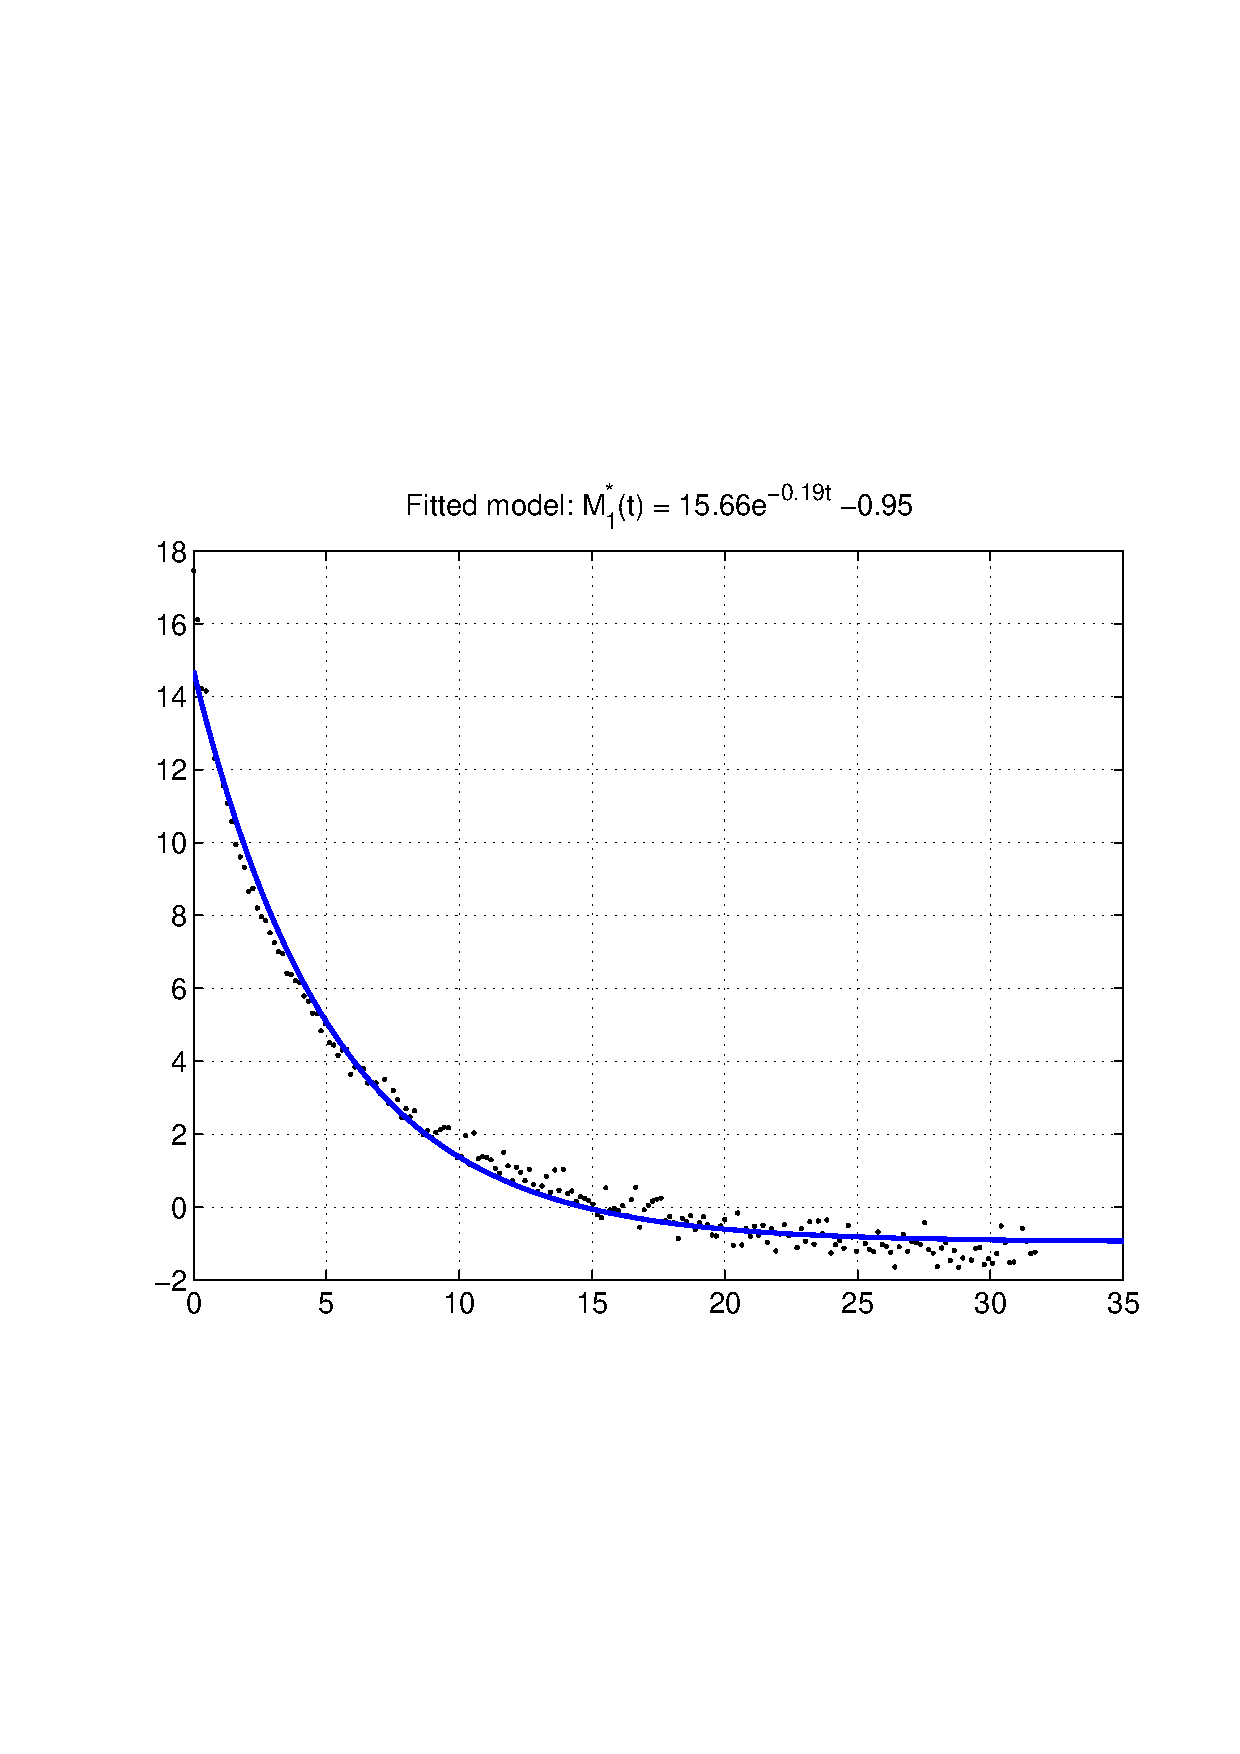
\includegraphics[width=70mm]{least-squares-model-1.pdf}} \quad \subfigure{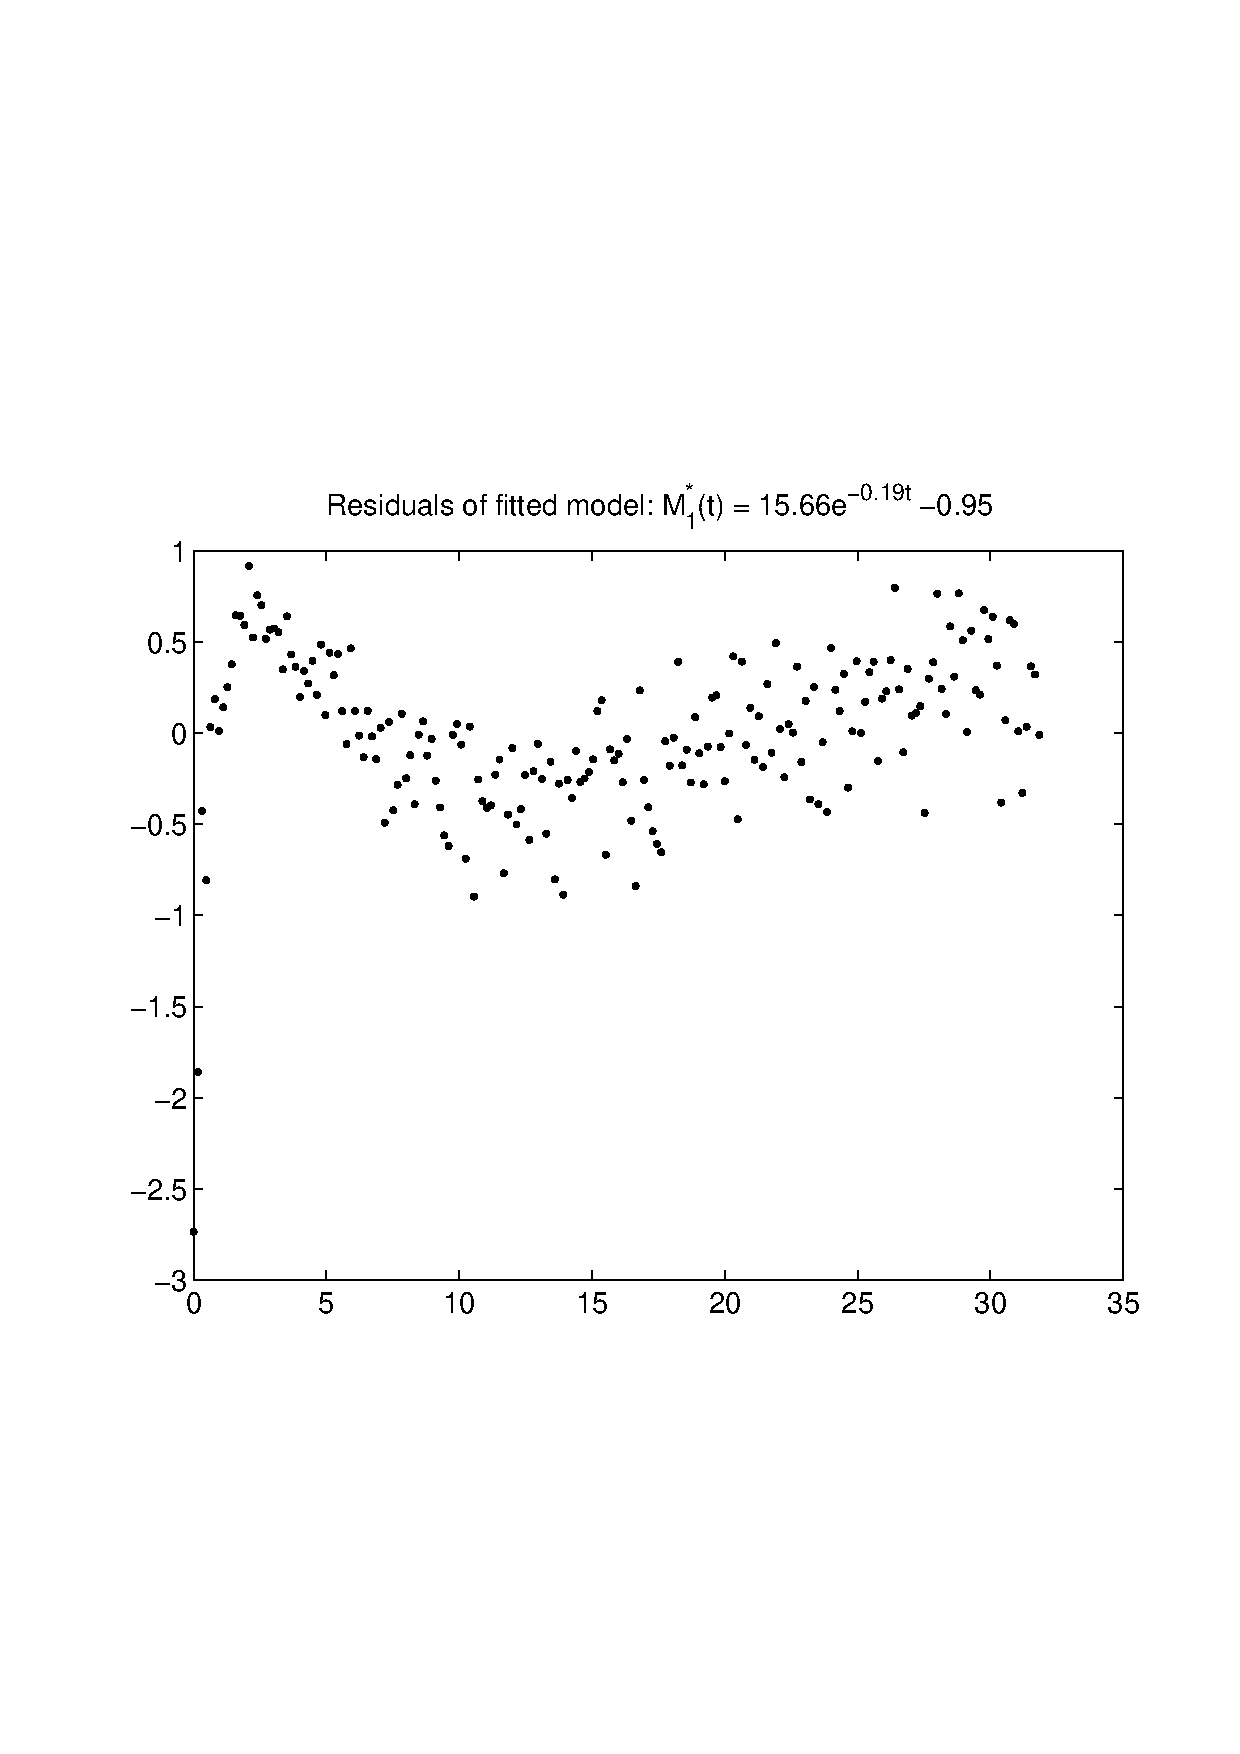
\includegraphics[width=70mm]{least-squares-model-1-res.pdf}}}
    \caption{Plot of fitted model and residuals for model given by (\ref{eq:model1})}
    \label{fig:model1-plots}
\end{figure}

\begin{tabular}{c c}
    Iteration & $\norm{\nabla f}$ \\\hline
    1 & 1.13e+03 \\ 
2 & 3.86e+01 \\ 
3 & 9.79e+01 \\ 
4 & 2.99e+01 \\ 
5 & 3.47e+01 \\ 
6 & 1.08e+01 \\ 
7 & 2.34e+00 \\ 
8 & 4.02e-01 \\ 
9 & 6.31e-02 \\ 
10 & 9.71e-03 \\ 
11 & 1.48e-03 \\ 
12 & 2.26e-04 \\ 
13 & 3.45e-05 \\ 
14 & 5.27e-06 \\ 
15 & 8.03e-07 \\ 
16 & 7.17e-08 \\ 

\end{tabular}
\begin{tabular}{c c}
    Iteration & $\norm{\nabla f}$ \\\hline
    1 & 4.99e+01 \\ 
2 & 3.65e+01 \\ 
3 & 2.86e+01 \\ 
4 & 2.18e+01 \\ 
5 & 1.97e+01 \\ 
6 & 1.95e+01 \\ 
7 & 1.95e+01 \\ 
8 & 1.95e+01 \\ 
9 & 1.95e+01 \\ 
10 & 1.95e+01 \\ 
11 & 1.95e+01 \\ 
12 & 1.95e+01 \\ 
13 & 1.95e+01 \\ 
14 & 1.95e+01 \\ 
15 & 1.95e+01 \\ 
16 & 1.95e+01 \\ 

\end{tabular}

\subsection*{Question 3.5}
Since the residuals of the previous model still showed some structure an extended model is now fitted. The model is given as
\begin{equation}\label{eq:model2}
    M_2(x, t) = x_3 e^{-x_1t} + x_4 e^{-x_2 t} + x_5
\end{equation}
To fit the model a starting guess needs to be found. Using the fitted $M_1$ model a good starting point could be 
\begin{equation*}
    \vecx^{(0)} = (0.2, 0.2, 8, 8, -1)^T
\end{equation*}
Using this starting guess a least squares fit for the new model is found using the \myverb{marquardt} function and the optimal model is found as
\begin{equation*}
    M_2^*(t) = 5.98e^{-0.87t} +12.29e^{-0.14t} -1.33
\end{equation*}
The new model is plotted along with the residuals of the model in figure~\ref{fig:model2-plots}

\begin{figure}
    \centering
    \mbox{\subfigure{\includegraphics[width=70mm]{least-squares-model-2.pdf}} \quad \subfigure{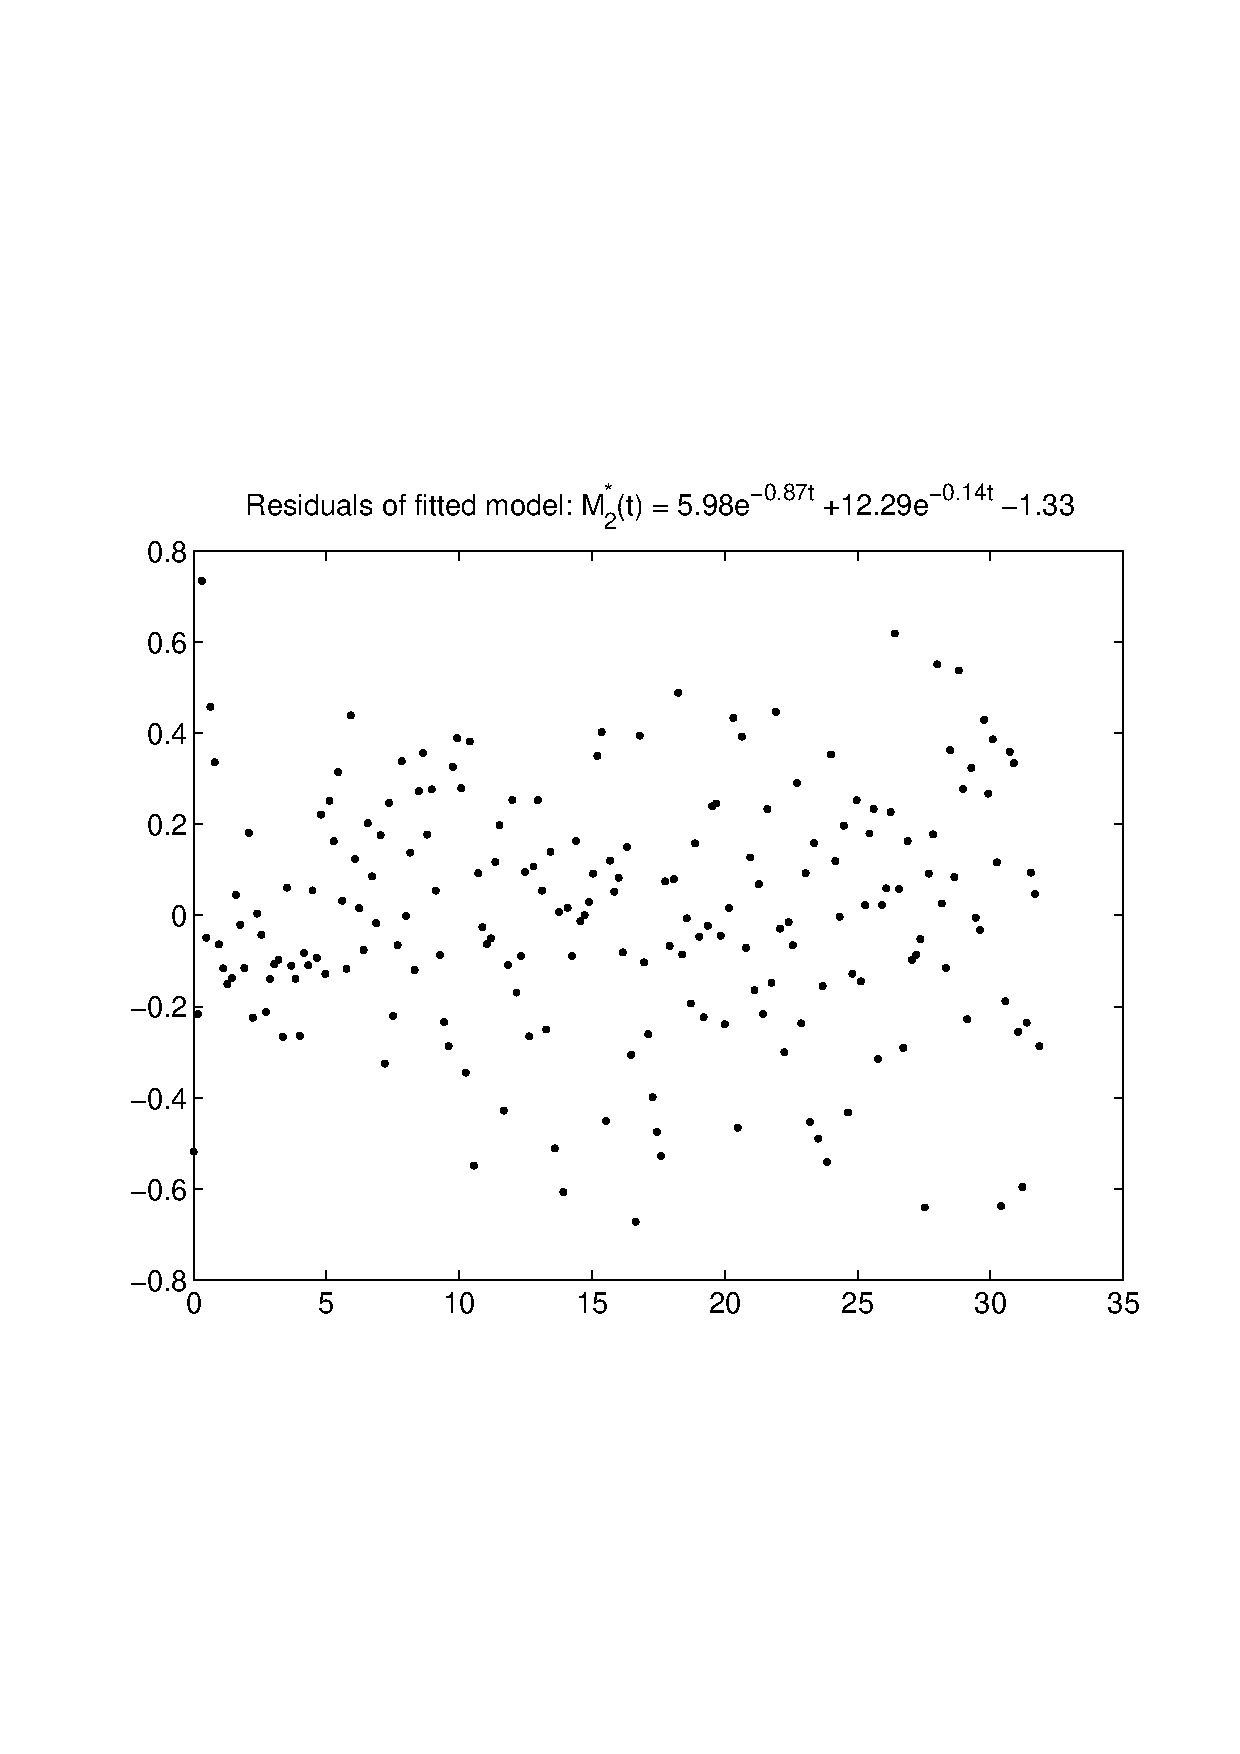
\includegraphics[width=70mm]{least-squares-model-2-res.pdf}}}
    \caption{Plot of fitted model and residuals for model given by (\ref{eq:model2})}
    \label{fig:model2-plots}
\end{figure}

\subsection*{Question 3.6}
From figure~\ref{fig:model2-plots} it is seen that the fit has improved overall compared with model $M_1$. The residuals looks much more like white noise which is expected for a well-fitted model. It is often assumed that the variance of the residuals is independent of the input $t$, but it is seen that the variance is smaller for $t\in[1;8]$ than for other $t$ values. This could maybe be fixed with a transformation of the data, but shouldn't be a big problem. Most importantly it is seen that the residuals center around a mean of 0 for all values of $t$. All in all the fit seems to be satisfactory for the data.

\section*{Question 4}

\subsection*{Question 4.1}

\end{document}
